\section*{Desarrollo}
    \subsection*{Desarrollo de la simulación}
    Para simular el proceso de producción de acetona vía alcohol isopropílico se propone una alimentación del 50\% respecto a la que una Turton et al en su proceso, así tenemos una alimentación de 25.98 kmol/h y fracciones mol de 0.67 IPA y 0.33 agua, a esta corriente (ALIM) se le une la corriente de circulación que sale por la parte de arriba de la segunda torre de destilación (DSTL-2) la cual contiene IPA y agua. Una vez que se han unido estas dos corrientes en un mezclador, la corriente resultante (S2) se alimenta al vaporizador (VAP) para pasar de una fase líquida a gas donde este opera 389 K y 2.6 atm. Después, esta corriente se alimenta al reactor donde este opera a 2atm y 636 K. Una vez que sale del reactor, la corriente pasa por dos intercambiadores de calor, uno que opera a 318 K y el otro a 293 K, ambos a 1 atm de presión. Ya que se enfri´´o la corriente, esta e alimenta a un tanque flash (FLASH) que opera a 1.5 atm y 293 K, de este sale una corriente de hidrógeno por la parte de arriba la cual se conecta a una torre de absoción (ABSOR), además a esta torre se alimenta una corriente de 10 kmol/h de agua. La corriente que sale por el fondo de la torre de absorción y el tanque flash, se mezclan y alimentan a la primer torre de destilación (DSTL-1), esta torre consta de 32 etapas (las cuales se determinaron previamente en una simulación con torres DSTWU), se alimenta en la etapa 17, opera a 1atm y tiene un condensador parcial-líquido-vapor con una relación de reflujo de 2.8 y una relación de destilado a alimentación de 0.45. La corriente que sale por la parte de arriba de la columna DSTL-1 (14) es la de mayor importancia ya que es la que contiene la acetona. La corriente que sale por el fondo de la columna DSTL-1 se alimenta a una segunda columna de destilación que consta de 3 etapas, alimentación en la etapa 2, condensador total, relación de reflujo de 0.845 y una relación de destilado a alimentación de 0.128 a 1 atm. La Figura \ref{fig:DiagramaCHIDO} muestra el diagrama general del proceso simulado en Aspen Plus especificando los equipos y corrientes del proceso.

        \begin{figure}[H]
            \centering
            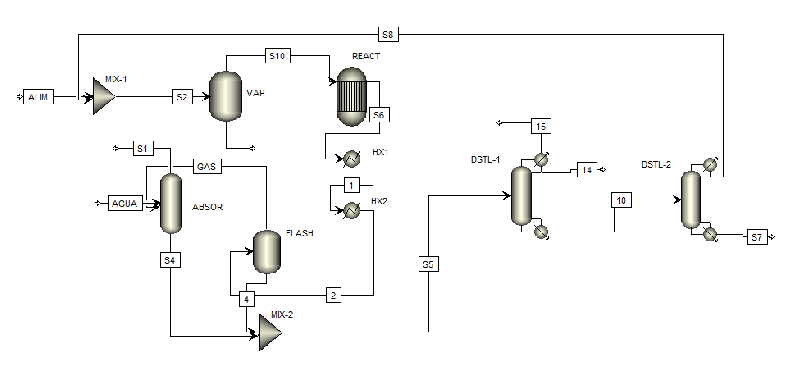
\includegraphics[width=16cm, height=8cm]{images/Diagramageneral.eps}
            \caption{Diagrama general del proceso simulado en Aspen Plus.}
            \label{fig:DiagramaCHIDO}
        \end{figure}

    \subsection*{Desarrollo del sistema de control}
    Para el sistema de control es necesario obtener la funciones transferencia a partir de las ecuaciones de balance de masa  del reactor además de los valores en estado estacionario  e iniciales.
    \paragraph{}
    Debido a que solo nos interesa la temperatura del flujo de entrada, nos centraremos en los balances para $A$, $T_r$ y $T_j$. Una vez que se tienen las ecuaciones se procede a linealizar las mismas.\\
    Se definen las variables de desviacion:\\
        $\Bar{C_A}= C_A - C_{As} $  ,  $\Bar{T}= T - T_s $  , $\Bar{T_j}= T_j - T_{js}$y $\Bar{F_j}= F_j - F_{js}$   


    \paragraph{}
    Los valores de nuestro sistema son:\\
        \begin{multicols}{2}
        %Para el calculos de las constantes
        \setlength{\parindent}{0cm}
        $F_{rs} = 0.0972\: m^3/s $\\ 
        $F_{j} = 0.01\: m^3/s$\\
        $k_0 = 3.51\: \times 10^5  1/s$ \\
        $UA = 1668431: J/s$\\
        $E = 72380\: J/mol\:K $\\
        $C_{pr} = 2500 \: J/Kg\:K$\\
        $C_{j} = 1700 \: J/Kg\:K$\\
        $ V_r = 3 \: m^3$\\
        $ V_j = 1 \: m^3$\\
        $ \Delta H_{rxn}= 70000 \:J/mol$\\
        $\rho_r = 785\:Kg/m^3$ \\
        $\rho_j = 970\:Kg/m^3$ \\
        $R = 8.314\: J/mol\: K$\\
        $T_s = 624\:K$\\
        $T_{j0} = 427\:K$\\
        $T_{j} = 327\:K$\\
        $C_{A0} = 526 \: mol/m^3$\\
        $C_{As} = 50.3168 \: mol/m^3$\\
        \end{multicols}

    Sustituyendo los valores en las ecuaciones \ref{balanceA}, \ref{energia} y \ref{energiachaqueta}, los balances quedan de la siguiente manera:\\

        $\dfrac{\partial (\ref{balanceA}) }{\partial C_A} = -\dfrac{F_r}{V_r}\Bar{C_A} = -0.0324\:\Bar{C_A}$

        $\dfrac{\partial (\ref{energia}) }{\partial C_A} = -\frac{\mathrm{\Delta H_{rxn}}\,\mathrm{k_0}\,{\mathrm{e}}^{-\frac{E}{R\,\mathrm{T_{rs}}}}}{\mathrm{C_{pr}}\,\mathrm{\rho_r}}\Bar{C_A}= - 0.0109 \:\Bar{C_A}$

        $\dfrac{\partial (\ref{energiachaqueta}) }{\partial C_A} = 0$

%% Para  Tr 

        $ \dfrac{\partial (\ref{balanceA}) }{\partial T_r} = -\frac{E\,\mathrm{k_0}\,{\mathrm{e}}^{-\frac{E}{R\,\mathrm{T_{rs}}}}}{R\,{\mathrm{T_{rs}}}^2}\Bar{T_r} = -0.0068 \:\Bar{T_r}$

        $ \dfrac{\partial (\ref{energia}) }{\partial T_r} = -\frac{F_r}{V_r}-\frac{\mathrm{UA}}{\mathrm{C_{pr}}\,V_r\,\mathrm{\rho_r}}-\frac{\mathrm{C_{As}}\,\mathrm{\Delta  H_{rxn}}\,E\,\mathrm{k_0}\,{\mathrm{e}}^{-\frac{E}{R\,\mathrm{T_{rs}}}}}{\mathrm{C{pr}}\,R\,{\mathrm{T_{rs}}}^2\,\mathrm{\rho_r}}\Bar{T_r}= -0.3281 \:\Bar{T_r}$

        $\dfrac{\partial (\ref{energiachaqueta}) }{\partial T_r} = \frac{\mathrm{UA}}{\mathrm{C_{pj}}\,\mathrm{V_j}\,\mathrm{\rho_j}}\Bar{T_r} = 1.0118  \:\Bar{T_r}$

%% Para  Tj

        $ \dfrac{\partial (\ref{balanceA}) }{\partial T_j} = 0$

        $ \dfrac{\partial (\ref{energia}) }{\partial T_j} =\frac{\mathrm{UA}}{\mathrm{C_{pr}}\,V_r\,\mathrm{\rho_r}} \Bar{T_j} = 0.2834 \:\Bar{T_j}$

        $ \dfrac{\partial (\ref{energiachaqueta}) }{\partial T_j} = -\frac{\mathrm{F_j}}{\mathrm{V_j}}-\frac{\mathrm{UA}}{\mathrm{C_{pj}}\,\mathrm{V_j}\,\mathrm{\rho_j}} \Bar{T_j} = -1.0218 \:\Bar{T_j}$

%% Para la  Vmanupulable
        $\dfrac{\partial (\ref{balanceA}) }{\partial F_j} = 0$

        $ \dfrac{\partial (\ref{energia}) }{\partial F_j} = 0$

        $ \dfrac{\partial (\ref{energiachaqueta}) }{\partial F_j} = -\frac{\mathrm{T_j}-\mathrm{T_j}_{0}}{\mathrm{V_j}}\Bar{F_j}= 88\Bar{F_j} $ \\
    En forma de matriz de  tiene:\\

        \begin{center}
            \begin{bmatrix}

            s + 0.0324 &   0.0068   &         0\\
            0.0109     & s + 0.3281 &   -0.2834\\
            0          &  - 1.0118  &  s+  1.0218\\ 
            \end{bmatrix}
            
            \begin{bmatrix}
            0\\
            0\\
            88
            \end{bmatrix}
        \end{center}
    \paragraph{}
    Realizando las transformadas de Laplace correspondiente se tiene que la funciones transferencia es:\\

        \begin{equation*}
            G(s) = \dfrac{88 s^2 + 31.72 s + 0.929}{s^{3} + 1.382\:s^2 + 0.09217\:s + 0.001495 }
        \end{equation*}
    Para proponer el controlador se va a utilizar el método de Cohen-Coon por ser un lazo abierto y además se agrega un escalón unitario para tener un delay, por lo tanto, para calcular los parámetros de los diferentes  controladores se utilizan las ecuaciones que se muestran en la \textit{Tabla \ref{tabla:ecucontrol}} . 

    %% Aqui se agregó una tabla 

    \begin{table}[H]
    \caption{ Ecuaciones para el calculo de los valores de distintos tipos de controladores por el método de Cohen-Coon} 
    \centering
    \begin{tabular}{llll}
    \hline
    Controlador & $K_c$ & $\tau_D$ & $\tau_I$  \\
    \hline
    P                   & $\frac{\tau}{K\:t_d}\left(1 +\frac{t_d}{3 \tau}  \right) $   & -   &-     \\
    PI                  & $\frac{\tau}{K\:t_d}\left(0.9 +\frac{t_d}{12 \tau}  \right) $   & $ t_d \frac{30 + 3(t_d/\tau)}{9+20(t_d/\tau)}$   &     \\
    PID                 &  $\frac{\tau}{K\:t_d}\left(4/3 +\frac{t_d}{4 \tau}  \right) $  & $ t_d \frac{32 + 6(t_d/\tau)}{13+8(t_d/\tau)}$   &  $ t_d \frac{4}{11+2(t_d/\tau)}$   \\
    \hline
    \end{tabular}
    \label{tabla:ecucontrol}
\end{table}


    donde $t_d$ es el delay,
    $K$ se calcula mediante: $B/S $ 
    donde $S$ es la pendiente a la tangente de la curva de reacciona lazo abierto y $B$ y el escalón en señal de control,$A$  es la magnitud del escalón. 

    \subsection*{Desarrollo de la viabilidad sustentable}
    En cuanto al objetivo de analizar el impacto económico, social y ambiental de la producción de acetona es necesario conocer las normas que regulan las concentraciones de acetona en distintos ambientes, descargas industriales en agua, suelo y aire. Así como los aspectos que alteren el entorno  social de los alrededores de la ubicación de la planta.
    El cumplimiento de los objetivos  para este proyecto es una serie de pasos para alcanzar la meta principal que es un análisis  de la producción de  acetona, tomando en cuenta que no solo este proceso afecta al sitio  donde se lleva a cabo la producción, si no que afecta  de diversas maneras a su entorno y a una parte de la sociedad

    \subsection*{Viabilidad sustentable económica}
    \subsubsection*{Importaciones y exportaciones de acetona}
    Las importaciones realizadas en los últimos 5 años vienen principalmente de Estados Unidos, Taiwán y Bélgica. En la \textit{Figura \ref{graf_acetona}} se muestran los respectivos porcentajes.

        \begin{figure}[H]
            \centering
            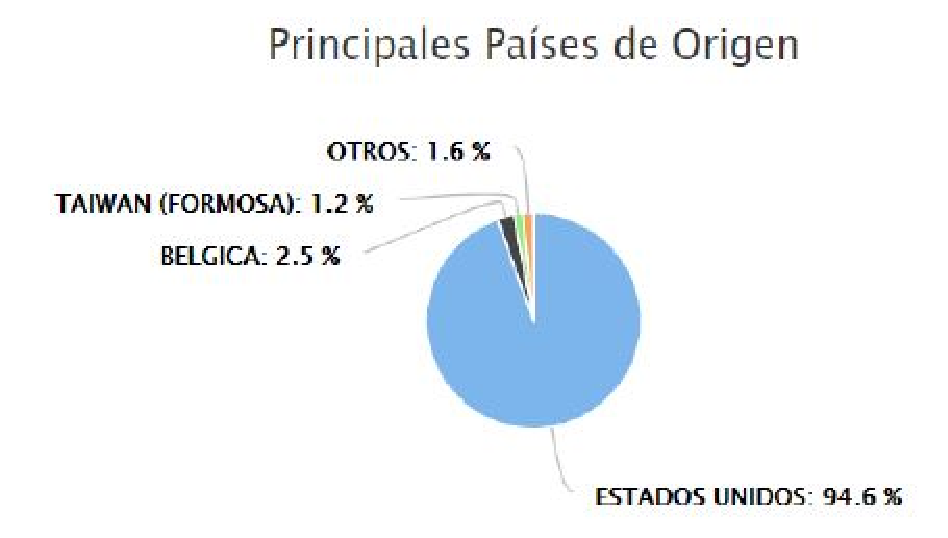
\includegraphics[scale= 0.7]{images/importacetona.eps}
            \caption{Origen importaciones acetona}
            \label{graf_acetona}
        \end{figure}

    Del 2015 al 2020 el valor de las importaciones a México asciende a \$ 351,868,389 USD y las exportaciones a \$ 13,166,844, cantidades que indican que las importaciones han sido mayores y esto indica que hay un amplio campo de aprovechamiento en la producción de acetona nacional para crecer en el mercado internacional.

    \subsubsection*{Capacidad de la planta}
    En México la producción de acetona cae en la categoría de producción de petroquímicos intermedios. El último dato que se encontró registrado por el INEGI de la capacidad instalada para producción de acetona fue en 2007 de 24,113 ton/año \cite{INEGI2009}
    %(INEGI, 2010).

    Con base al estudio de mercado y tomando en cuenta las tendencias de consumo se estima que la capacidad de la planta sería de 6,660.2 ton/año de acetona, cubriendo, un 18.5\% de la producción anual de acetona estimada en el 2020 según las tendencias de demanda y crecimiento de este producto.

    Se establece que el tiempo de operación anual es de 300 días al año y operando un proceso continuo de 24 horas al día, se alcanzará una producción de 22.2 toneladas al día, que será la capacidad nominal de los equipos que se utilizaran en la planta.

    La capacidad se establece basándose en plantas ya existentes productoras de acetona, tomando en cuenta que una sobreproducción nacional puede causar pérdidas económicas.
    \subsubsection*{Costos de los equipos}

    Para calcular la sustentabilidad económica del proyecto utilizamos el \textbf{análisis económico de Aspen} el cual nos calcula los costos de los equipos, servicios, instalación y operación del proyecto, estos se muestran en las Tablas \ref{tab:equipos}, \ref{tab:servicios}, \ref{tab:serviciosxaño}, \ref{tab:manodeobra} y \ref{tab:resultados} en la sección de resultados, cabe destacar que la acetona se vende aproximadamente en $2.00$ USD por kg.

    \subsection*{Viabilidad sustentable ambiental}

    \subsubsection*{Aguas residuales}

    La corriente que sale por el fondo de la segunda torre de destilación es la única que contiene ''agua residual'', sin embargo, gracias a la tecnología seleccionada y al elevado porcentaje de rendimiento donde se obtiene un producto de alta pureza, esta corriente tiene una fracción mol de 0.9961 agua, por lo tanto, con un adecuado sistema es posible recircularla a nuestro proceso.

    \subsubsection*{Residuos atmosféricos}

    Los principales contaminantes atmosféricos que se pueden producir en planta son:\\

    \textbf{Emisiones directas}\\

    Son producidas en el reactor donde se producen vapores orgánicos volátiles cetónicos o alcohólicos, estos pueden ser tratados en una columna de desorción de gases donde se recupere materia prima o producto principal emitiendo gases al ambiente con el límite máximo permisible.\\

    \textbf{Emisiones indirectas}\\

    Son las que produce la combustión de gas natural, es un combustible más limpio que los combustibles derivados de petróleo. Una solución es alimentar aire en exceso para evitar las combustiones incompletas que emiten compuestos nitrogenados, sulfúricos, etc.


    \subsection*{Viabilidad sustentable social}
    La acetona es un solvente esencial para la industria cosmética y del cuidado personal. Se espera que el rápido crecimiento de la industria del cuidado personal en los países en desarrollo impulse la demanda del mercado de acetona. Se prevé que la industria mundial del cuidado personal crezca con una tasa compuesta anual de casi el 5,78\% en los próximos años. Las economías emergentes, como los países de Asia-Pacífico y América Latina, tienen un enorme potencial de crecimiento para la industria del cuidado personal.

